\chapter{Theoretical Background}

\section{Magnetic Field of a Single Circular Coil}

\begin{figure}[h]
\centering
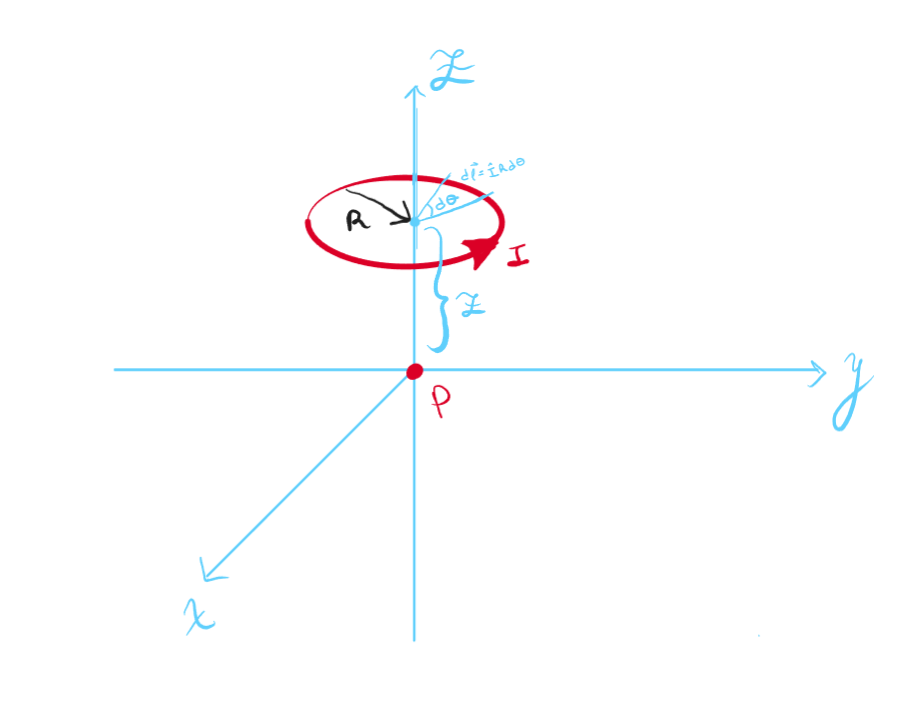
\includegraphics[width=0.5\textwidth]{assets/single-coil-magnetic-field-hand-drawn.png}
\caption{Magnetic field of a single circular coil.}
\end{figure}

The magnetic field $\vec{B}$ at point $P$ due to a current $I$ flowing through a circular coil of radius $R$ can be calculated using the Biot-Savart law:

\begin{align*} 
    d\vec{B} &= \frac{\mu_0 I}{4\pi} \frac{d\vec{l} \times \vec{r}}{|\vec{r}|^3} \\
\end{align*}

\noindent Where:
\begin{itemize}
    \item $\mu_0$ is the permeability of free space.
    \item $d\vec{l}$ is the differential length element of the coil.
    \item $\vec{r}$ is the position vector from the differential element to the point $P$.
\end{itemize}

\newpage
\thispagestyle{plain}

To find the magnetic field at point $P$ due to any radius $r$ and any arc length $l$, we can integrate the differential magnetic field over the specified arc length:

\begin{align*}
    &d\vec{l} = \hat{\theta}rd\theta \\
    &\vec{r} = -\hat{R}r -\hat{k}z \\
    &|\vec{r}| = \sqrt{r^2 + z^2} \\
    &\Rightarrow \vec{B}(r, \theta, z) = \int\limits_0^\theta d\vec{B}(r, \theta', z) \\
    &= \int\limits_0^\theta \frac{\mu_0 I r}{4\pi}\cdot(r^2 + z^2)^{-\frac{3}{2}}\cdot\left[\hat{\theta}rd\theta' \times (-\hat{R}r - \hat{k}z)\right] \\
    &\boxed{\vec{B}(r, \theta, z) = \frac{\mu_0 I r \theta}{4\pi} \cdot(r^2 + z^2)^{-\frac{3}{2}} \cdot (\hat{k}r - \hat{R}z)} \\
\end{align*}

And for a full circular coil with radius $R$ and distance from center $z$, the magnetic field is:

\begin{align*}
    \vec{B}(R, 2\pi, z) = \frac{\mu_0 I R 2\pi}{4\pi} \cdot(R^2 + z^2)^{-\frac{3}{2}} \cdot (\hat{k}R - \hat{R}z) \\
    \boxed{\vec{B}(R, 2\pi, z) = \frac{\mu_0 I R}{2} \cdot(R^2 + z^2)^{-\frac{3}{2}} \cdot (\hat{k}R - \hat{R}z)} \\
\end{align*}


\section{Magnetic Field with Coil of N Turns}

For coils with \( N \) turns, the magnetic field is simply multiplied by \( N \):

\[ \boxed{\vec{B}(R, 2\pi, z) = \frac{\mu_0 I R N}{2} \cdot(R^2 + z^2)^{-\frac{3}{2}} \cdot (\hat{k}R - \hat{R}z)} \]

\newpage{}
\thispagestyle{plain}

\section{Helmholtz Coil Configuration}

\begin{figure}[h]
    \centering  
    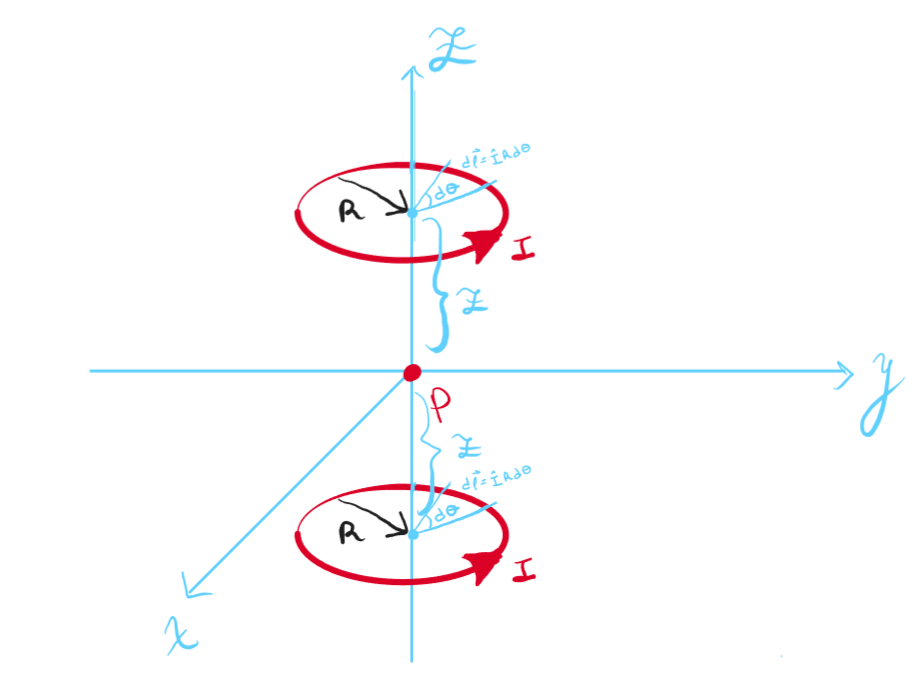
\includegraphics[width=0.5\textwidth]{assets/helmholtz-coil-setup-hand-drawn.png}
    \caption{Helmholtz coil configuration.}
    \end{figure}

For two identical coils of radius \( R \) separated by a distance \( d \) and carrying current \( I \), the magnetic field at point \( P \) is:

\begin{align*}
    \vec{B}_{\text{total}} &= \vec{B}_{\text{top}} + \vec{B}_{\text{bottom}} \\
    let~\xi(r, \theta) &= \frac{\mu_{0}Ir\theta N}{4\pi} \\
    \vec{B}_{Bottom}(r,\theta,z) &=\xi(r, \theta)\bigg[\frac{\hat{k}r+\hat{R}(z-d/2)}{(r^2+(z-d/2)^2)^{3/2}}\bigg] \\
    \vec{B}_{Top}(r,\theta,z) &=\xi(r, \theta)\bigg[\frac{\hat{k}r-\hat{R}(z+d/2)}{(r^2+(z+d/2)^2)^{3/2}}\bigg] \\
    \vec{B}_{Total}(r,\theta,z) &=\xi(r, \theta)\bigg[\frac{\hat{k}r+\hat{R}(z-d/2)}{(r^2+(z-d/2)^2)^{3/2}}+\frac{\hat{k}r-\hat{R}(z+d/2)}{(r^2+(z+d/2)^2)^{3/2}}\bigg] \\
\end{align*}

To achieve maximum uniformity at the center (\( z = 0 \)), we need to find the optimal ratio of \( d/R \).

\newpage{}
\thispagestyle{plain}

\section{Optimal Distance \( d \)}
To find the optimal distance \( d \), we need to minimize the second derivative of \( \vec{B}_{\text{total}}(R, 2\pi, z) \) at \( z = 0 \). This ensures that the magnetic field is as uniform as possible.

\begin{align*}
    \text{let}~\xi(R) &= \hat{k}2\pi \mu_0 I R^2 \\
    \vec{B}_{total}(R, 2\pi, z) &= \xi(R) \cdot \frac{1}{(R^{2}+z^{2})^{3/2}} \\
    \implies \vec{B}_{total}(R, 2\pi, \delta z) &= \xi(R) \cdot \bigg[\frac{1}{(R^{2}+(\frac{d}{2}-\delta z)^{2})^{3/2}} + \frac{1}{(R^{2}+(\frac{d}{2}+\delta z)^{2})^{3/2}}\bigg] \\ 
    \frac{\partial^{2} \vec{B}_{total}}{\partial (\delta z)^{2}} &= \xi(R) \bigg[\frac{\frac{15}{4}(d-2\delta z)^{2}}{(R^{2}+\frac{1}{4}(d-2\delta z)^{2})^{7/2}}-\frac{3}{(R^{2}+\frac{1}{4}(d-2\delta z)^{2})^{5/2}} \\ 
    &\quad -\frac{3}{(R^{2}+\frac{1}{4}(d+2\delta z)^{2})^{5/2}}+\frac{\frac{15}{4}(d-2\delta z)^{2}}{(R^{2}+\frac{1}{4}(d+2\delta z)^{2})^{7/2}}\bigg] \\ 
    \lim_{\delta z \to 0} \frac{\partial^{2} \vec{B}_{total}}{\partial (\delta z)^{2}} &= \xi(R) \bigg[\frac{\frac{15}{2}d^{2}}{(R^{2}+\frac{d^{2}}{4})^{7/2}}-\frac{6}{(R^{2}+\frac{d^{2}}{4})^{5/2}}\bigg] = 0 \\ 
    &\implies \frac{15d^{2}}{R^2+\frac{d^{2}}{4}} = 12 \\
    &\implies 15d^{2} = 12R^{2} + 3d^{2} \\
    &\implies 12d^{2} = 12R^{2} \\
    &\implies d^{2} = R^{2} \\
    &\implies d = R ~ \text{(neither $d$ nor $R$ can be negative)} \\
\end{align*}

\noindent Where:

\begin{itemize}
    \item \( d \) is the distance between the coils.
    \item \( z \) is the distance from the center of the coils.
    \item \( \delta z \) is a small change in \( z \).
    \item \( \xi(R) \) is the radius dependent coefficent.
\end{itemize}

This means that the optimal distance between the coils is equal to the radius of the coils.

\newpage{}
\thispagestyle{plain}

\section{Partial Derivatives}

\begin{align*}
    \frac{\partial \vec{B}}{\partial \theta} &= \frac{\mu_{0} Ir N}{4\pi}\Big[\frac{(\hat{k}r-\hat{R}(z+r/2))}{(r^2+(z+r/2)^2)^{3/2}}+\frac{(\hat{k}r+\hat{R}(z-r/2))}{(r^2+(z-r/2)^2)^{3/2}}\Big] \\
    \frac{\partial \vec{B}}{\partial r} &= \frac{\mu_{0} I\theta N}{4\pi}\Bigg[\frac{(2\hat{k}r-\hat{R}(2+r))}{(r^2+(z+r/2)^2)^{3/2}} -\frac{3(\hat{k}r^2 -\hat{R}(2r+r^2/2))(2r+(z+r/2))}{2(r^2+(z+r/2)^2)^{5/2}} \\
    & +\frac{(2\hat{k}r-\hat{R}(2-r))}{(r^2+(z-r/2)^2)^{3/2}}-\frac{3(\hat{k}r^2 +\hat{R}(2r-r^2/2))(2r-(z-r/2))}{2(r^2+(z-r/2)^2)^{5/2}}\Bigg] \\
    \frac{\partial \vec{B}}{\partial z} &= \frac{\mu_{0} Ir\theta N}{4\pi}\Big[\frac{-\hat{R}}{2(r^2+(z+r/2)^2)^{3/2}}-\frac{3(z+r/2)(\hat{k}r-\hat{R}(z+r/2))}{(r^2+(z+r/2)^2)^{5/2}} \\
    & -\frac{\hat{R}}{2(r^2+(z-r/2)^2)^{3/2}}-\frac{(z-r/2)(\hat{k}r+\hat{R}(z-r/2))}{3(r^2+(z-r/2)^2)^{5/2}}\Big] \\
\end{align*}
